\noindent\textbf{We get:}
\begin{align*}
	\frac{\partial c_1^\ast}{\partial t}=D\frac{\partial^2 c_1^\ast}{\partial x^2}-\nu_1^-(x,t)\\
	\frac{\partial c_n^\ast}{\partial t}=D\frac{\partial^2 c_n^\ast}{\partial x^2}+\nu_n^+(x,t)-\nu_n^-(x,t)\quad n=2,\ldots ,N
\end{align*}
where $\nu_n^+,\nu_n^-$ are the activation and deactivation rates, respectively\vspace{0.1cm}\\
\textbf{Boundary conditions}
\begin{align*}
	-D\frac{\partial c^\ast_1}{\partial x}\Big|_{x=0}&=\nu_1^+ \frac{\partial c_1^\ast}{\partial x}\Big|_{x=L}&=0\\
	\frac{\partial c_n^\ast}{\partial x}\Big|_{x=0}=&0=\frac{\partial c_n^\ast}{\partial x}\Big|_{x=L} &,n=2,3,\ldots ,N
\end{align*}
Assuming Michaelis-Menten Kinetics for the cascade, we have
\begin{equation*}
	\nu_n^-=V_n^-\frac{c_n^\ast(x,t)}{k_n^-+c_n^\ast(x,t)};\quad v_1^+=V_1^+ \frac{c_1^\text{tot}-c_1^{\ast}(0,t)}{k_1+c_1^\text{tot}-c_1^\ast(0,t)}
\end{equation*}
\begin{equation*}
	\nu_n^+=V_n^+c_{n-1}^\ast(x,t)\frac{c_n^\text{tot}-c_n^\ast(x,t)}{k_n^+c_n^\text{tot}-c_n^\ast(x,t)}\qquad n=2,3,\ldots ,N
\end{equation*}
We assume now that all parameters are independent of the cascade level
\begin{align*}
	k_n^-=k^-,V_n^-=V^-\qquad c_n^\text{tot}=c^\text{tot}\qquad n=1,2,\ldots ,N\\
	\text{and } k_n^+=k^+;\qquad v_n^+c_\text{tot}=v^+ \qquad \text{for } n=2,3,\ldots ,N
\end{align*}
We assume small concentrations (linear Michaelis-Menten regime)\\
Nondimensionalising the equations by setting
\begin{equation*}
	C_n=\frac{c_n^\ast}{c^\text{tot}};\quad x'=\sqrt{\frac{k_-}{D}}x;\quad t'=k_+t;\quad \gamma=\frac{k'_-}{k'_+}; \text{ with } k'_\pm=\frac{V_\pm}{k_\pm}
\end{equation*}
and dropping primes for $x,k$ and $t$ gives
\begin{align*}
	\partial_t C_1=\gamma\frac{\partial^2 C_1}{\partial x^2}-\gamma C_1\\
	\partial_t C_n=\gamma \partial_x^2C_n-\gamma C_n+(1-C_n)C_{n-1}
\end{align*}
\textbf{Boundary equations}
\begin{align*}
	-\partial_x C_1|_{x=0}&=\nu(1-C_1(x=0)); & D\partial_x C_1|_{x=L}&=0\\
	\partial_x C_n|_{x=0}=&0=\partial_x C_n|_{x=L} & n=2,3,\ldots &,N\\
	\nu&=\frac{\nu_1^+}{k_1^+}\sqrt{\frac{1}{Dk_{-1}}}
\end{align*}
The important parameter is $\gamma$, i.e. the ratio between deactivation and activation rates
\begin{enumerate}[label={$(\roman*)$}]
	\item $\gamma < 1$ The signal propagates into the system
	\item $\gamma > 1$ Localisation at the membrane
\end{enumerate}
\begin{figure}[H]
	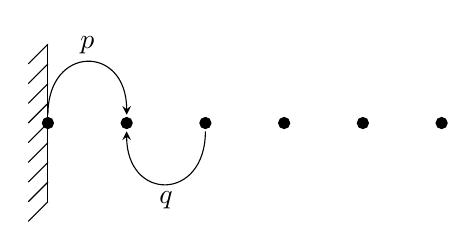
\begin{tikzpicture}
		\foreach \x in {0,...,5}{
			\draw[fill=black] (\x,0)circle(2pt)coordinate(A\x);
		}
		\draw (0,-1)--(0,1);
		\foreach \y in {-1,-0.75,...,1.2}{
			\draw (-0.25,{\y-0.25})--(0,\y);
		}
		\draw[->,>=stealth,shorten <= 3pt, shorten >= 3pt] (A0) .. controls +(0,1) and +(0,1) .. (A1)node[midway,above]{$p$};
		\draw[->,>=stealth,shorten <= 3pt, shorten >= 3pt] (A2) .. controls +(0,-1) and +(0,-1) .. (A1)node[midway,below]{$q$};
	\end{tikzpicture}\hspace{2cm}
	\begin{tikzpicture}[>=stealth]
		\node at (-1,-1){$p<q$};
		\draw[->] (0,-2.5)--(0,0.5)node[above left]{$\log(x)$};
		\draw[->] (0,0)--(2.5,0)node[below left]{$t$};
		\draw (0,0)--(2,-2);
	\end{tikzpicture}
\end{figure}
\noindent The stationary state of the system can be obtained for $y>1$. As in the fingle level model we get
\begin{equation*}
	C_1(x)=C_1(0)e^{-x}\qquad (\text{boundary control})
\end{equation*}
The approximate recurrence relation (neglecting $C_nC_{n-1}$) then reads:
\begin{equation*}
	\gamma\frac{d^2C_n}{dx^2}-\gamma C_n+C_{n-1}=0
\end{equation*}
This can be solved by the polynomial ansatz
\begin{equation*}
	C_n(x)=\left(\sum\limits_{m=0}^{n-1}Q_n^{(m)}x^m\right)e^{-x}\quad \text{for } \gamma>1
\end{equation*}
For $\gamma <1$ this solution breaks down near $x=0$. Nevertheless we get
\begin{equation*}
	C_n(x)\approx \frac{C_1(0)}{(n-1)!(2\gamma)^{n-1}}x^{n-1}e^{-x}
\end{equation*}
for the tail of the profile
\subsubsection{Theory of Turing Pattern Formation}
Two-component system in two dimensions. Chemical concentrations $u(\vec{x},t)$ and $v(\vec{x},t)$ with $\vec{x}\in\mathbb{R}^2\ \left(=\begin{pmatrix} x\\ y\end{pmatrix}\right)$, $t\in\mathbb{R}^+$. We assume an area $\Omega$ where $0\leq x \leq L$, $0\leq y\leq L$.\\
The standard reaction-diffusion (RD) model takes the form:
\begin{align*}
	\frac{\partial u}{\partial t}&=D_u\nabla^2u +f(u,v)\\
	\frac{\partial v}{\partial t}&=D_v\nabla^2v+f(u,v)
\end{align*}
The nonlinear functions $f,g$ describe the chemical reactions, $D_v,D_u$ the diffusion for the two species. No flux boundary conditions
\begin{equation*}
	\vec{n}\cdot\vec{\nabla}u=0=\vec{n}\cdot\vec{\nabla} v\qquad for \vec{x}\in\partial\Omega
\end{equation*}
$\vec{n}$ denotes the outward normal on the boundary.\\
We assume that there exists a homogeneous stationary state $(u^*,v^\ast)$ for which $f(u^\ast,v^\ast)=g(u^\ast,v^\ast)=0$\vspace{1mm}\\
\textbf{\underline{\smash{Turing's idea}}}: Stable stationary state in absence of diffusion, unstable in presence of diffusion. We linearize the equations ($*$) about the homogeneous state $(u^*,v^*)$ by setting $U=u-u^*,\ V=v-v^*$
\begin{equation*}
	\frac{\partial}{\partial t}\begin{pmatrix} U\\ V \end{pmatrix} = \mathbb{L}\begin{pmatrix}U\\ V\end{pmatrix}=\begin{pmatrix}f_u&f_v\\ g_u&g_v\end{pmatrix}_{u^*,v^*}\begin{pmatrix}U\\ V\end{pmatrix}+\begin{pmatrix}D_u&0\\ 0&D_v\end{pmatrix}\begin{pmatrix}\nabla^2 U\\\nabla^2 V\end{pmatrix}
\end{equation*}
with $f_x=\frac{\partial f}{\partial x}$
